\section{实验:研究凸透镜成像}\label{sec:1-7}

凸透镜能够使物体成像,物体离凸透镜的距离不同,所成的像也不同。
我们做实验来研究凸透镜成像的各种情况。

实验可以在如图 \ref{fig:1-26} 所示的光具座上进行。用蜡烛火焰作为物体,
研究它发出的光通过焦距已知的凸透镜后在光屏上所成的像。

\begin{figure}[htbp]
    \centering
    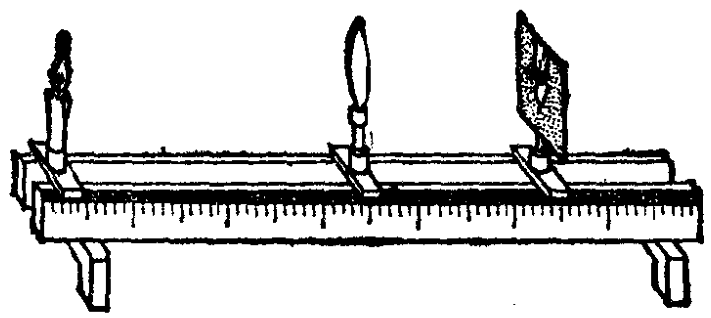
\includegraphics[width=0.7\textwidth]{../pic/czwl2-ch1-26}
    \caption{}\label{fig:1-26}
\end{figure}

在光具座上由左向右依次放置蜡烛、凸透镜和光屏。为了使烛焰的像能成在光屏的中间,
要调整凸透镜和光屏的高度,使它们的中心跟烛焰的中心大致在同一高度。

先调整凸透镜的位置,使蜡烛到凸透镜的距离(简称为物距,用 $u$ 来表示)大于凸透镜焦距的二倍(即 $u > 2f$)。

沿光具座移动光屏,直到光屏上出现清晰的烛焰像为止。
观察光屏上的像是倒立的还是正立的,是放大的还是缩小的。
测出像到凸透镜的距离(简称为像距,用 $v$ 来表示),把这时的像距跟焦距、二倍焦距相比较。
把观察和测量、比较的结果填入下面的表里。

\begin{tblr}{
    hlines, vlines, stretch=1.3,
    colspec={Q[c,8em]ccQ[c,8em]},
    cells={valign=m},
}
    \SetCell[r=2]{c}{物距 \\ ($u$)} & \SetCell[c=2]{c}{像的性质} & & \SetCell[r=2]{c}{像距 \\ ($v$)} \\
    & 倒立或成立 & 放大或缩小 & \\
    $u > 2f$ & & & \\
    $2f > u >f$ & & & \\
\end{tblr}

再向左移动凸透镜的位置,减小物距,使蜡烛位于二倍焦距与焦点间($2f > u >f$),照上一段要求的那样,
移动光屏,在光屏上得到清晰的烛焰像,进行观察和测量、比较,把结果填入上面表里。

蜡烛位于焦点以外,物距不断减小的过程中,像距怎样变?像的大小怎样变?

如果继续向左移动凸透镜的位置,使蜡烛位于焦点以内($u < f$),移动光屏,在光屏上能不能得到烛焰像?
从光屏这一侧透过凸透镜观察烛焰,能看到一个正立、放大的烛焰像吗?

